\documentclass[11pt]{article}
\usepackage[T1]{fontenc}
\usepackage[utf8]{inputenc}
\usepackage{enumerate}
\usepackage{setspace}
\usepackage{amsmath,amssymb,amsthm}
\usepackage{graphicx}
\usepackage{bbm}
\usepackage[round]{natbib}
\usepackage[nohead]{geometry}
\usepackage[bottom]{footmisc}
\usepackage{indentfirst}
\usepackage{endnotes}
\usepackage{graphicx}%
\usepackage{eurosym}
\usepackage{array}
\usepackage{booktabs}
\usepackage{caption}
\usepackage{subcaption}
\usepackage{rotating}
% \usepackage[hidelinks]{hyperref}
\usepackage{floatrow} %[capposition=top]
\floatsetup{footposition=bottom,capposition=top}
\renewcommand{\labelitemi}{--}
\renewcommand{\labelitemii}{$\bullet$}
\bibliographystyle{chicago}
% \geometry{left=1in,right=1in,top=1.00in,bottom=1.0in}
\let\olditemize\itemize
\renewcommand{\itemize}{
  \olditemize
  \setlength{\itemsep}{-1pt}
}

\begin{document}

\title{Competition between physicians: evidence from Paris\ \\ \ \\(Very preliminary)}
\author{Etienne Chamayou\thanks{e-mail:
\textit{etienne.chamayou@ensae.fr}}\medskip\\{\normalsize CREST and Department of Economics, Ecole Polytechnique }}
\maketitle

\sloppy%

\onehalfspacing

\textbf{Abstract:}

This note compares the locations and prices of general practitioners and ophtalmologists in Paris and its suburbs. Prices of general practitioners are largely regulated, hence the only way to increase income for most of them is to increase the number of patients, and thus to chose location based on healthcare demand and offer. Conversely, virtually all ophtalmologists are free to set prices. They can thus increase revenue through higher fees, which gives them an incentive to settle in wealthier areas. The comparison of geographic distributions and prices show that they do so in a significant way while it is not the case for general practictioners.

\strut

\textbf{Keywords:}

\strut

\textbf{JEL Classification Numbers:} XXX

\pagebreak%
\doublespacing

\section{Introduction}

The lack of physicians is a most prominent health policy issue in France. Among the various specialities, ophtalmology is one of the most affected, which translates into a high deregulation i.e. a high proportion of physicians free to set prices. On the other hand, most general practictioners are constrained to adopt the very same fee, determined by law. While the debate certainly belongs in the public sphere, the complexity of the regulation and the lack of data make it difficult to develop a reasonable opinion. An element which most likely limits our ability to reform the system is the absence of consensus as to whether healthcare should be viewed as a market or not. Data studied in this note suggest that ophtalmologists do respond to market incentives by focusing on wealthier areas where they set higher fees.

\section{Data}

\section{GPs}

\begin{figure}[H]
    \caption{Density of GPs vs. household revenue by district}
	\centering
		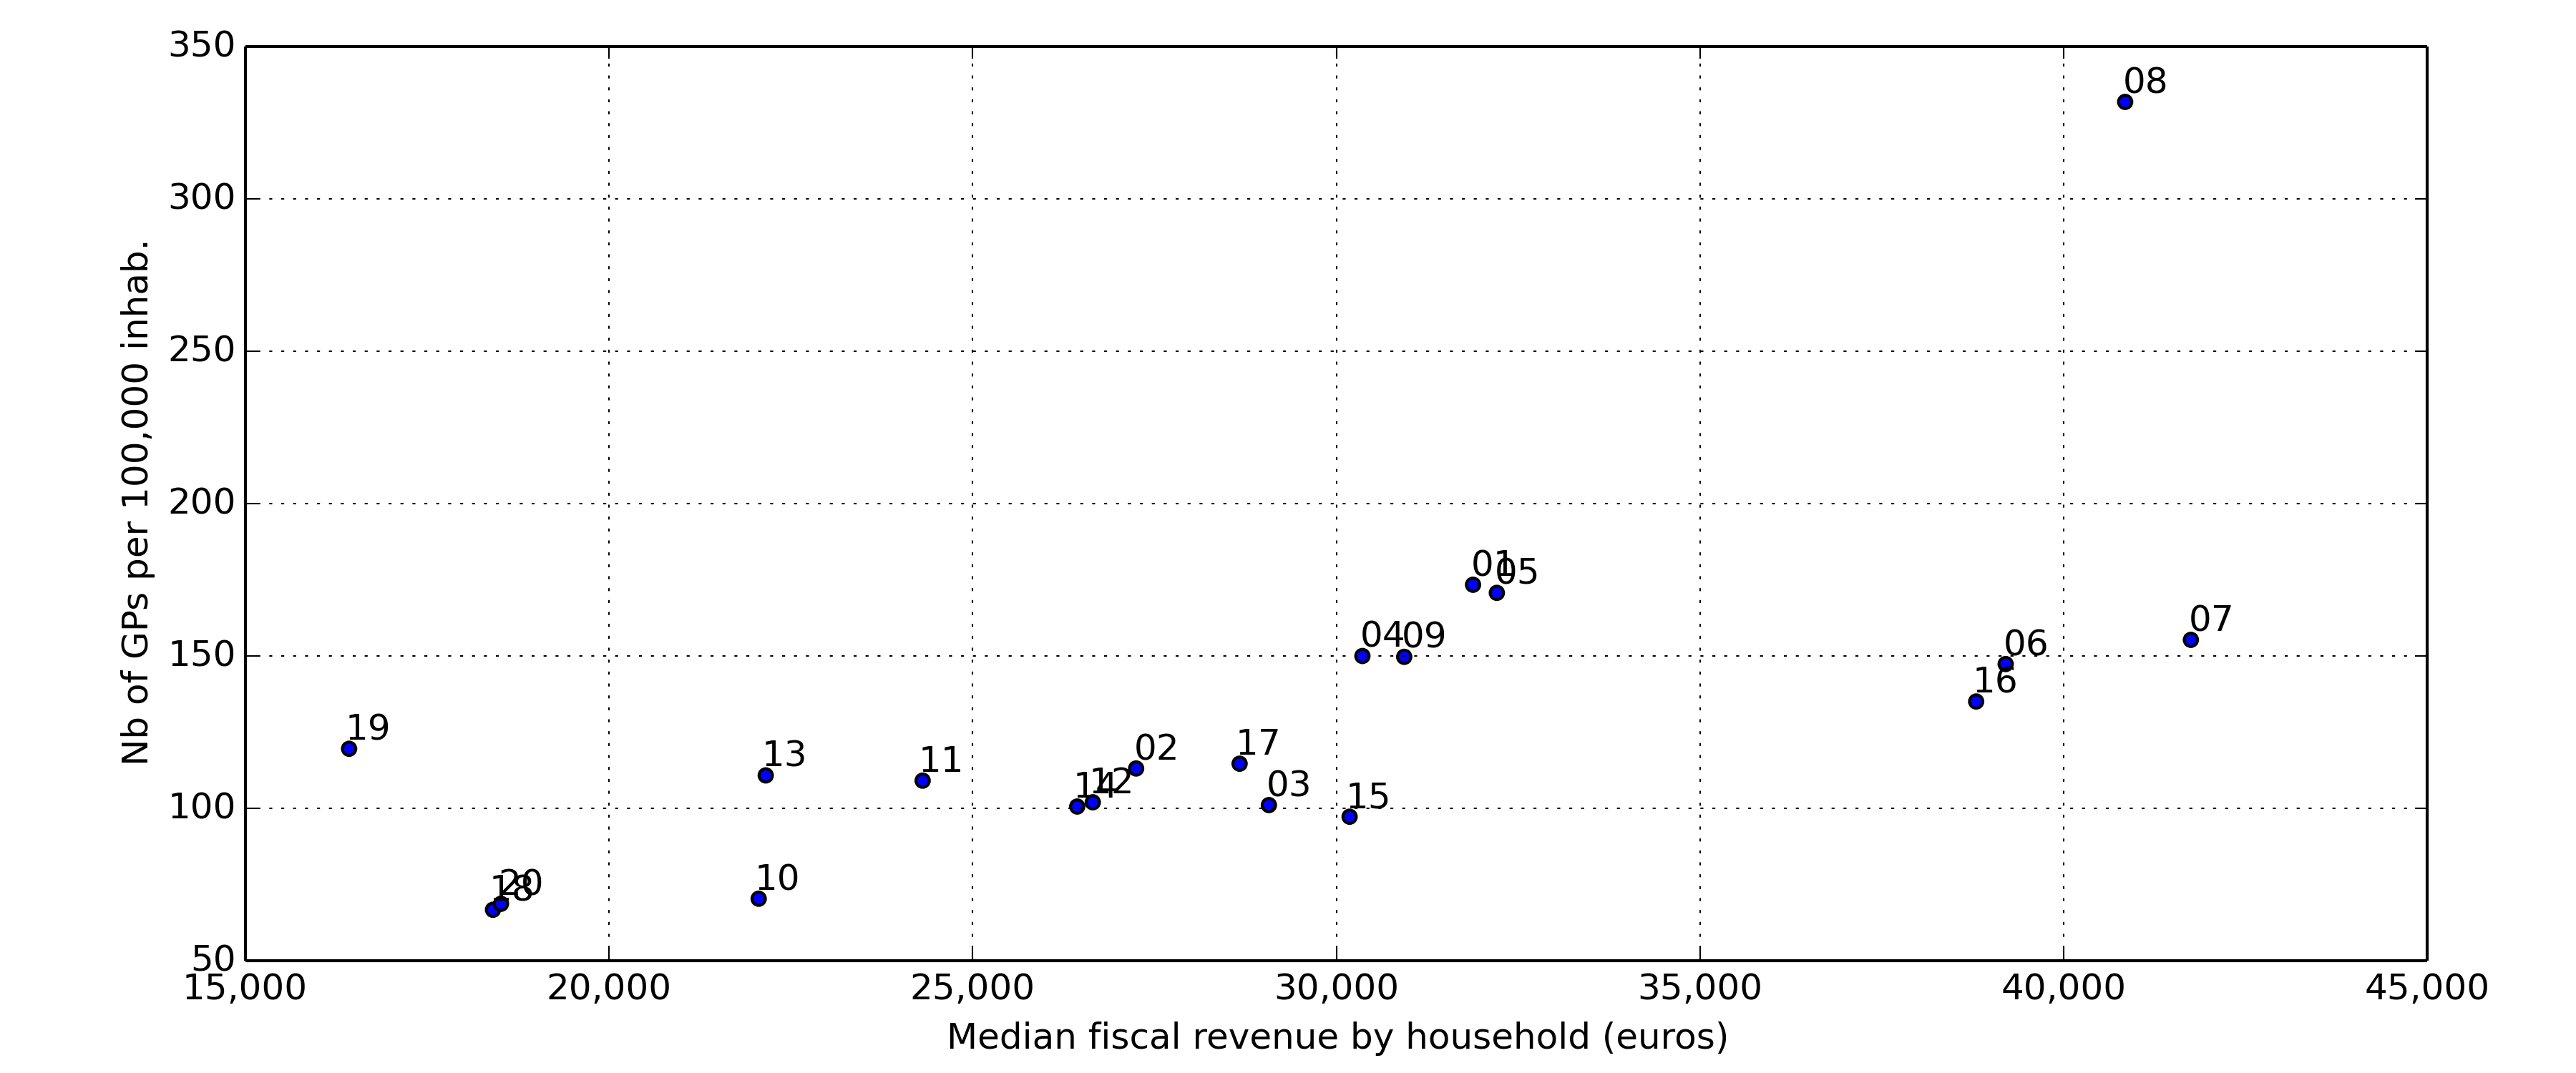
\includegraphics[width=16cm]{images/GP_Ardt_DensityVsRevenue.png}
\end{figure}

\begin{figure}[H]
    \caption{Density of sector 1 GPs vs. household revenue by district}
	\centering
		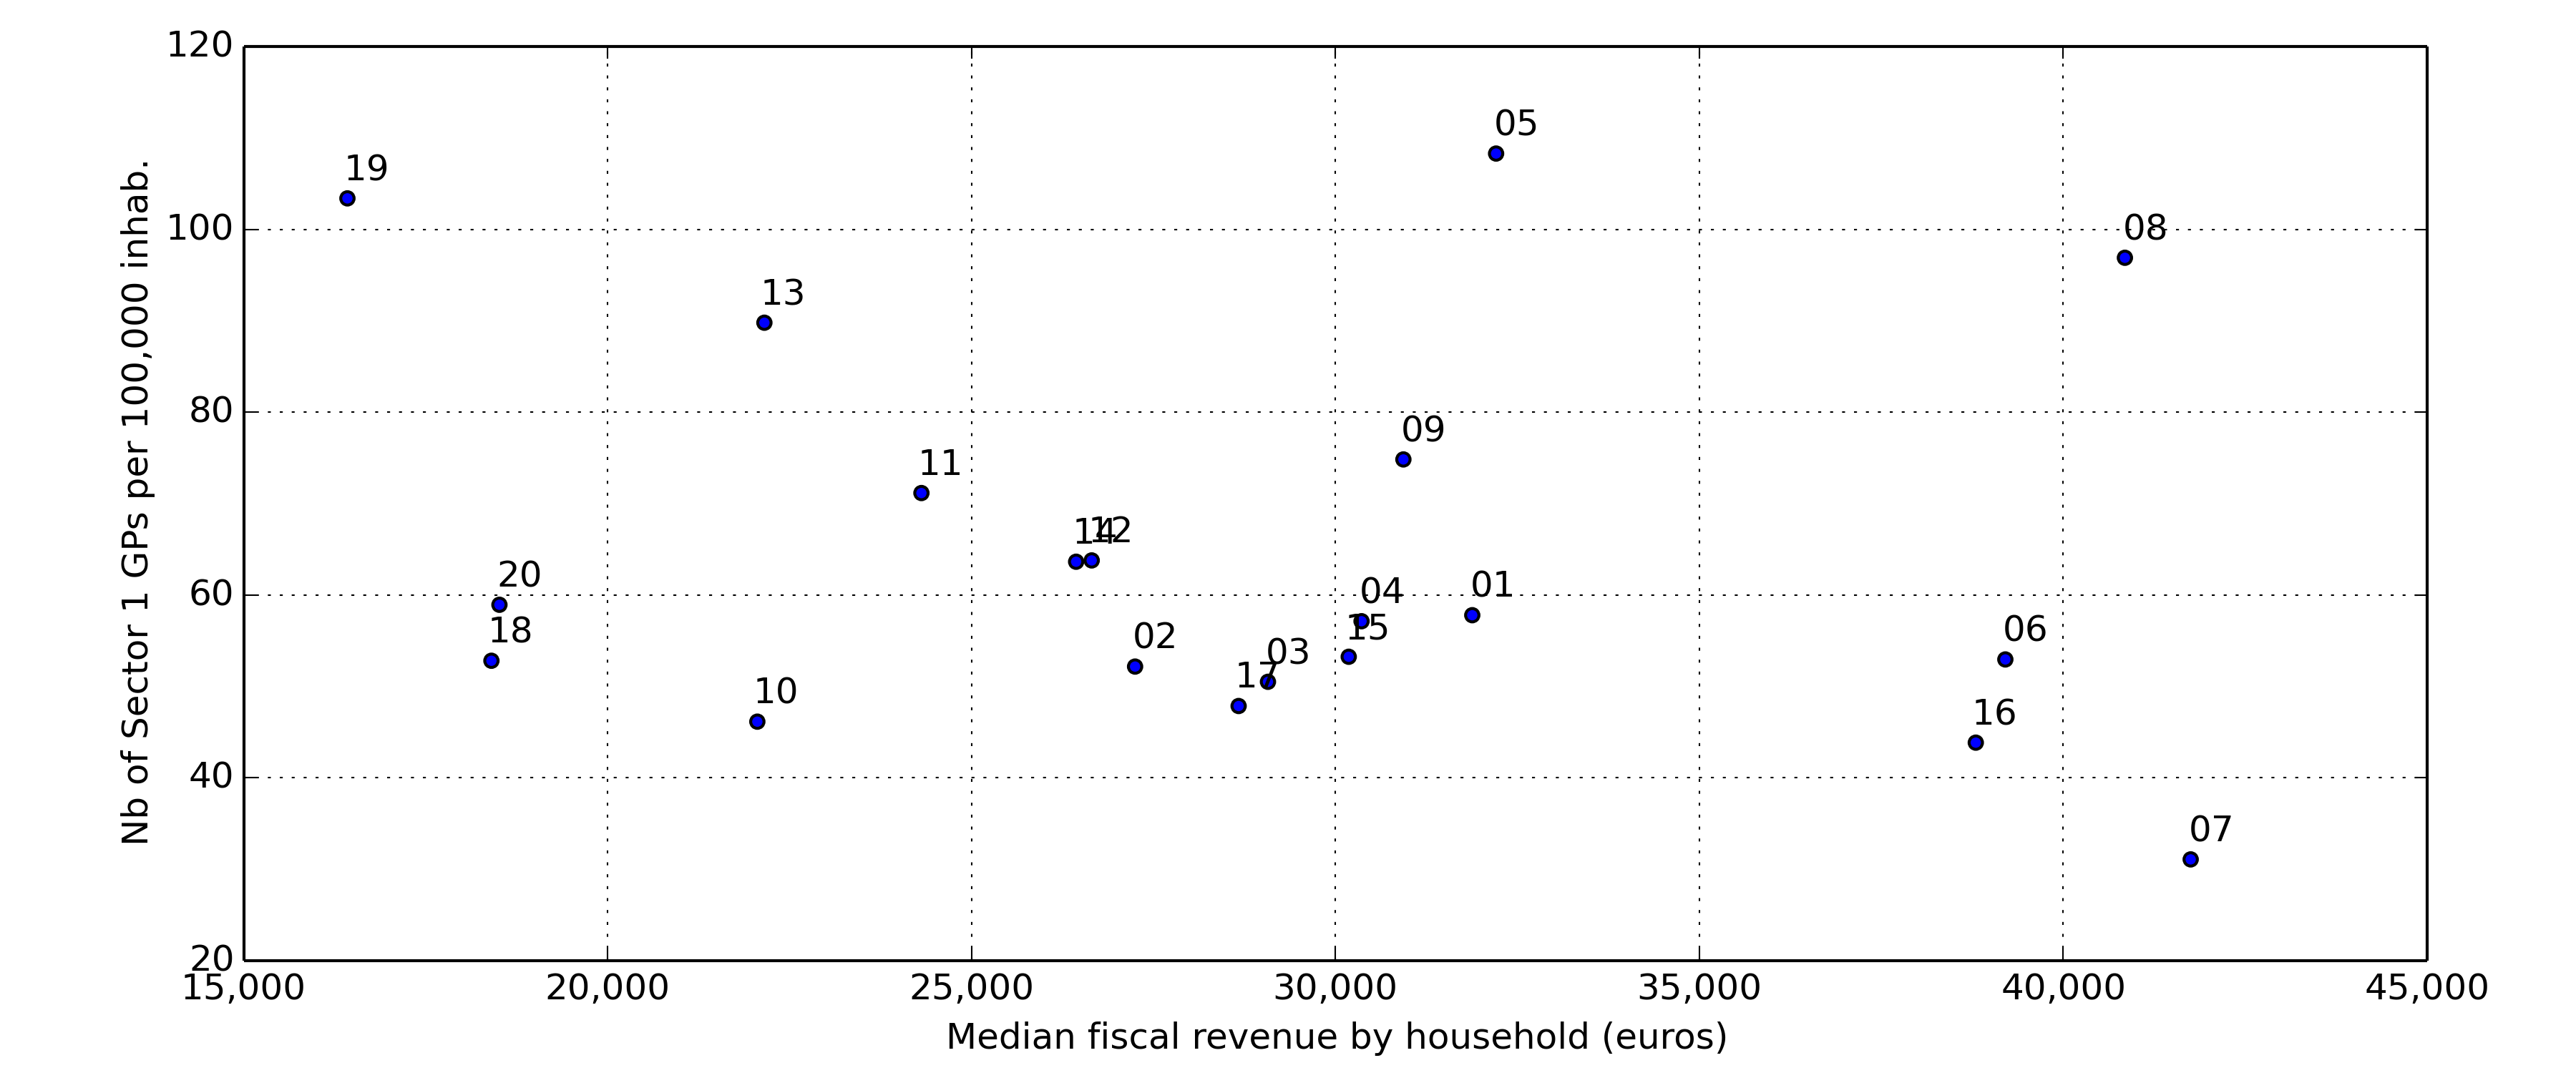
\includegraphics[width=16cm]{images/GP_Ardt_DensityS1VsRevenue.png}
\end{figure}

\begin{figure}[H]
    \caption{Density of sector 2 GPs vs. household revenue by district}
	\centering
		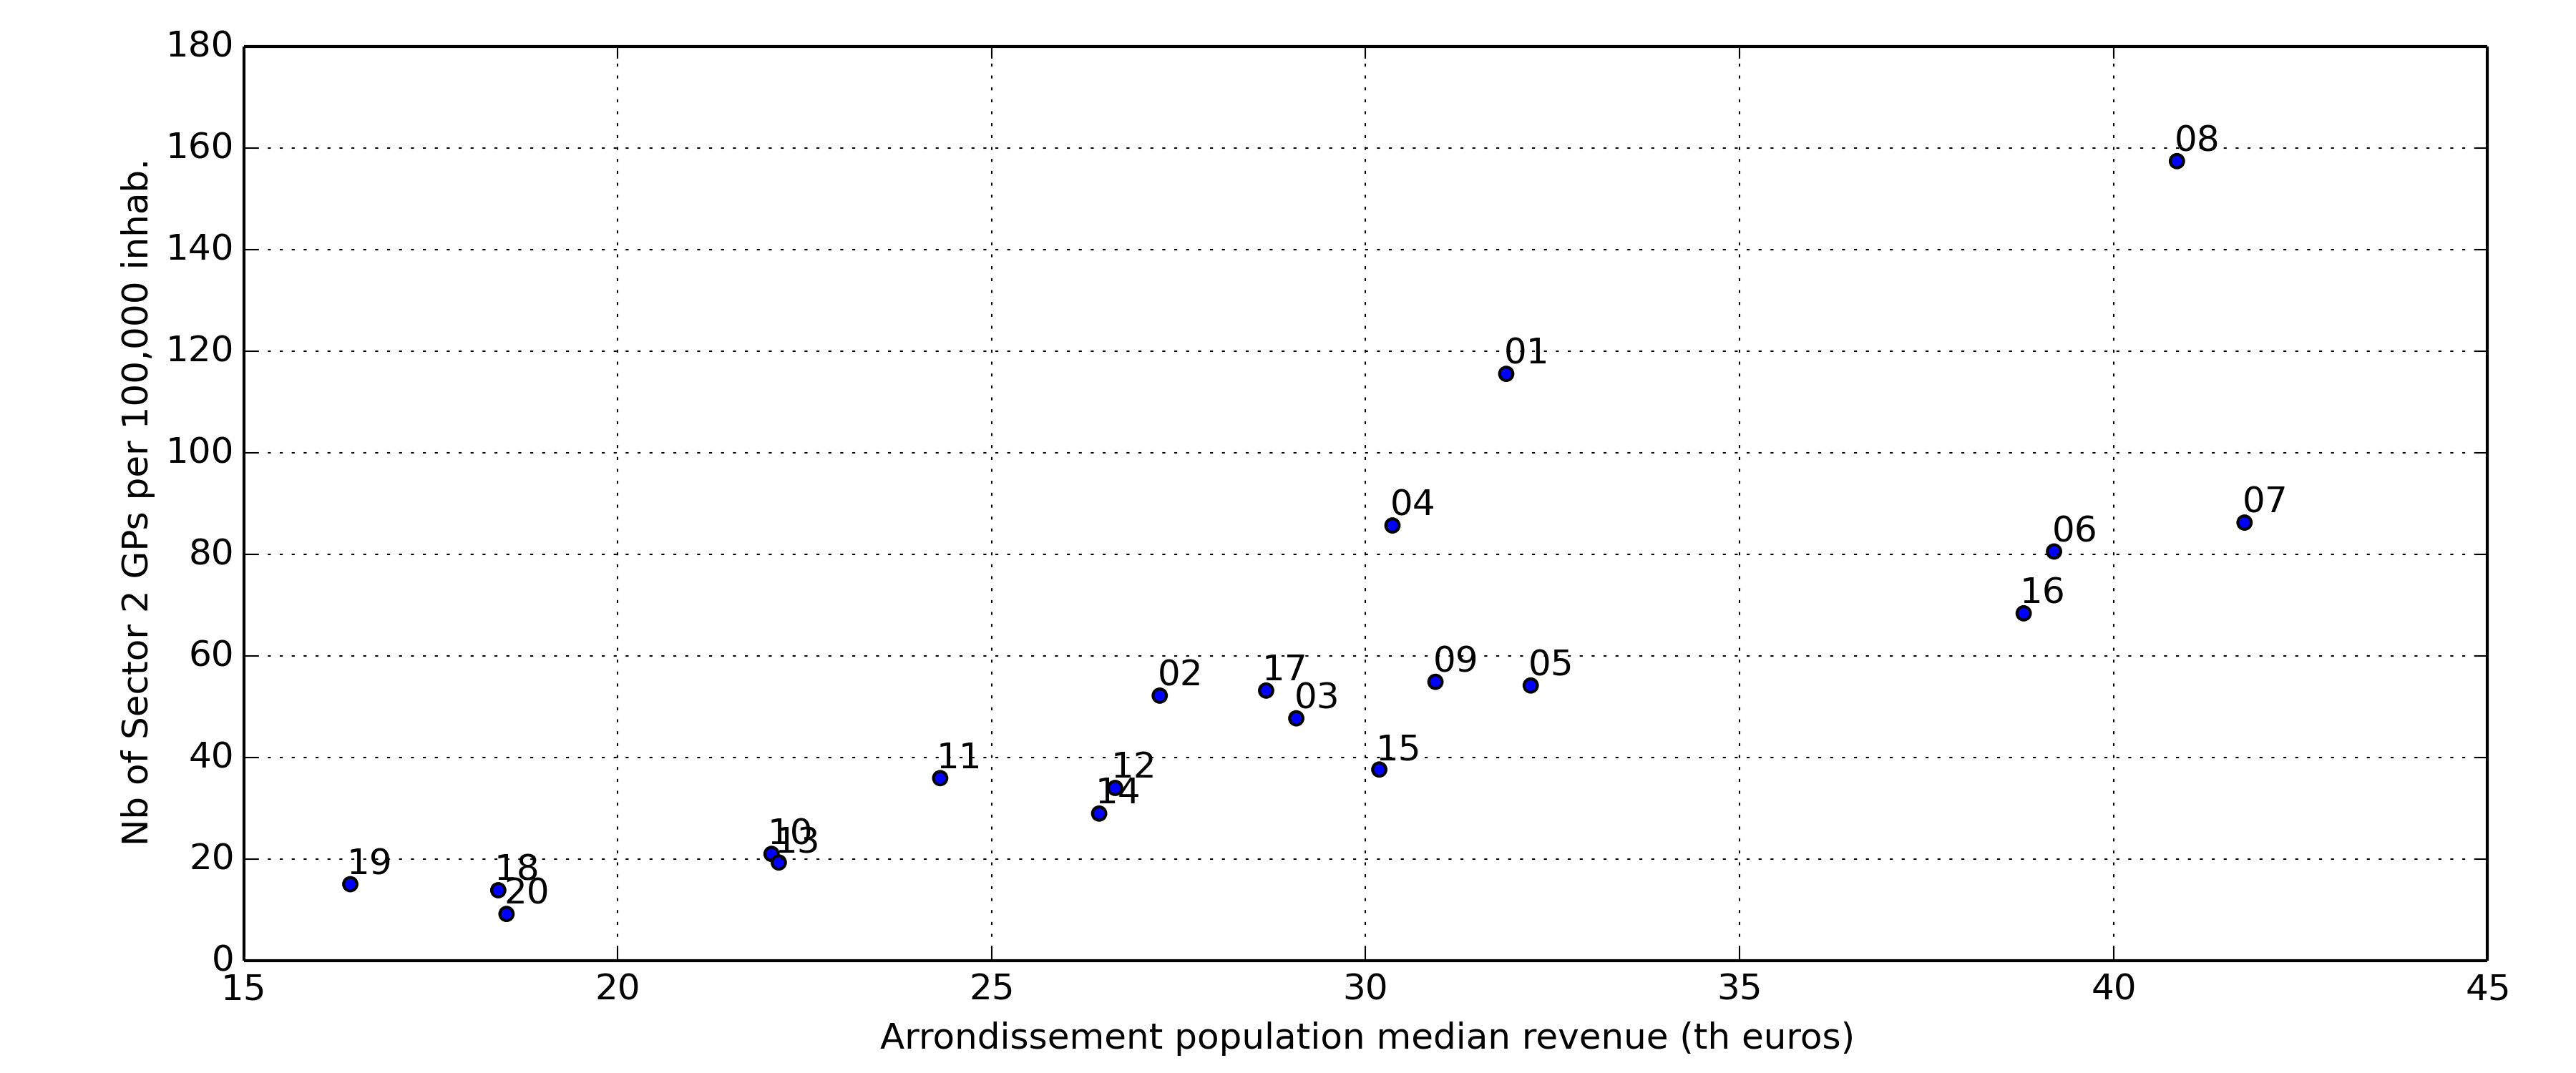
\includegraphics[width=16cm]{images/GP_Ardt_DensityS2VsRevenue.png}
\end{figure}

\begin{figure}[H]
    \caption{Average sector 2 GP consultation price vs. household revenue by district}
	\centering
		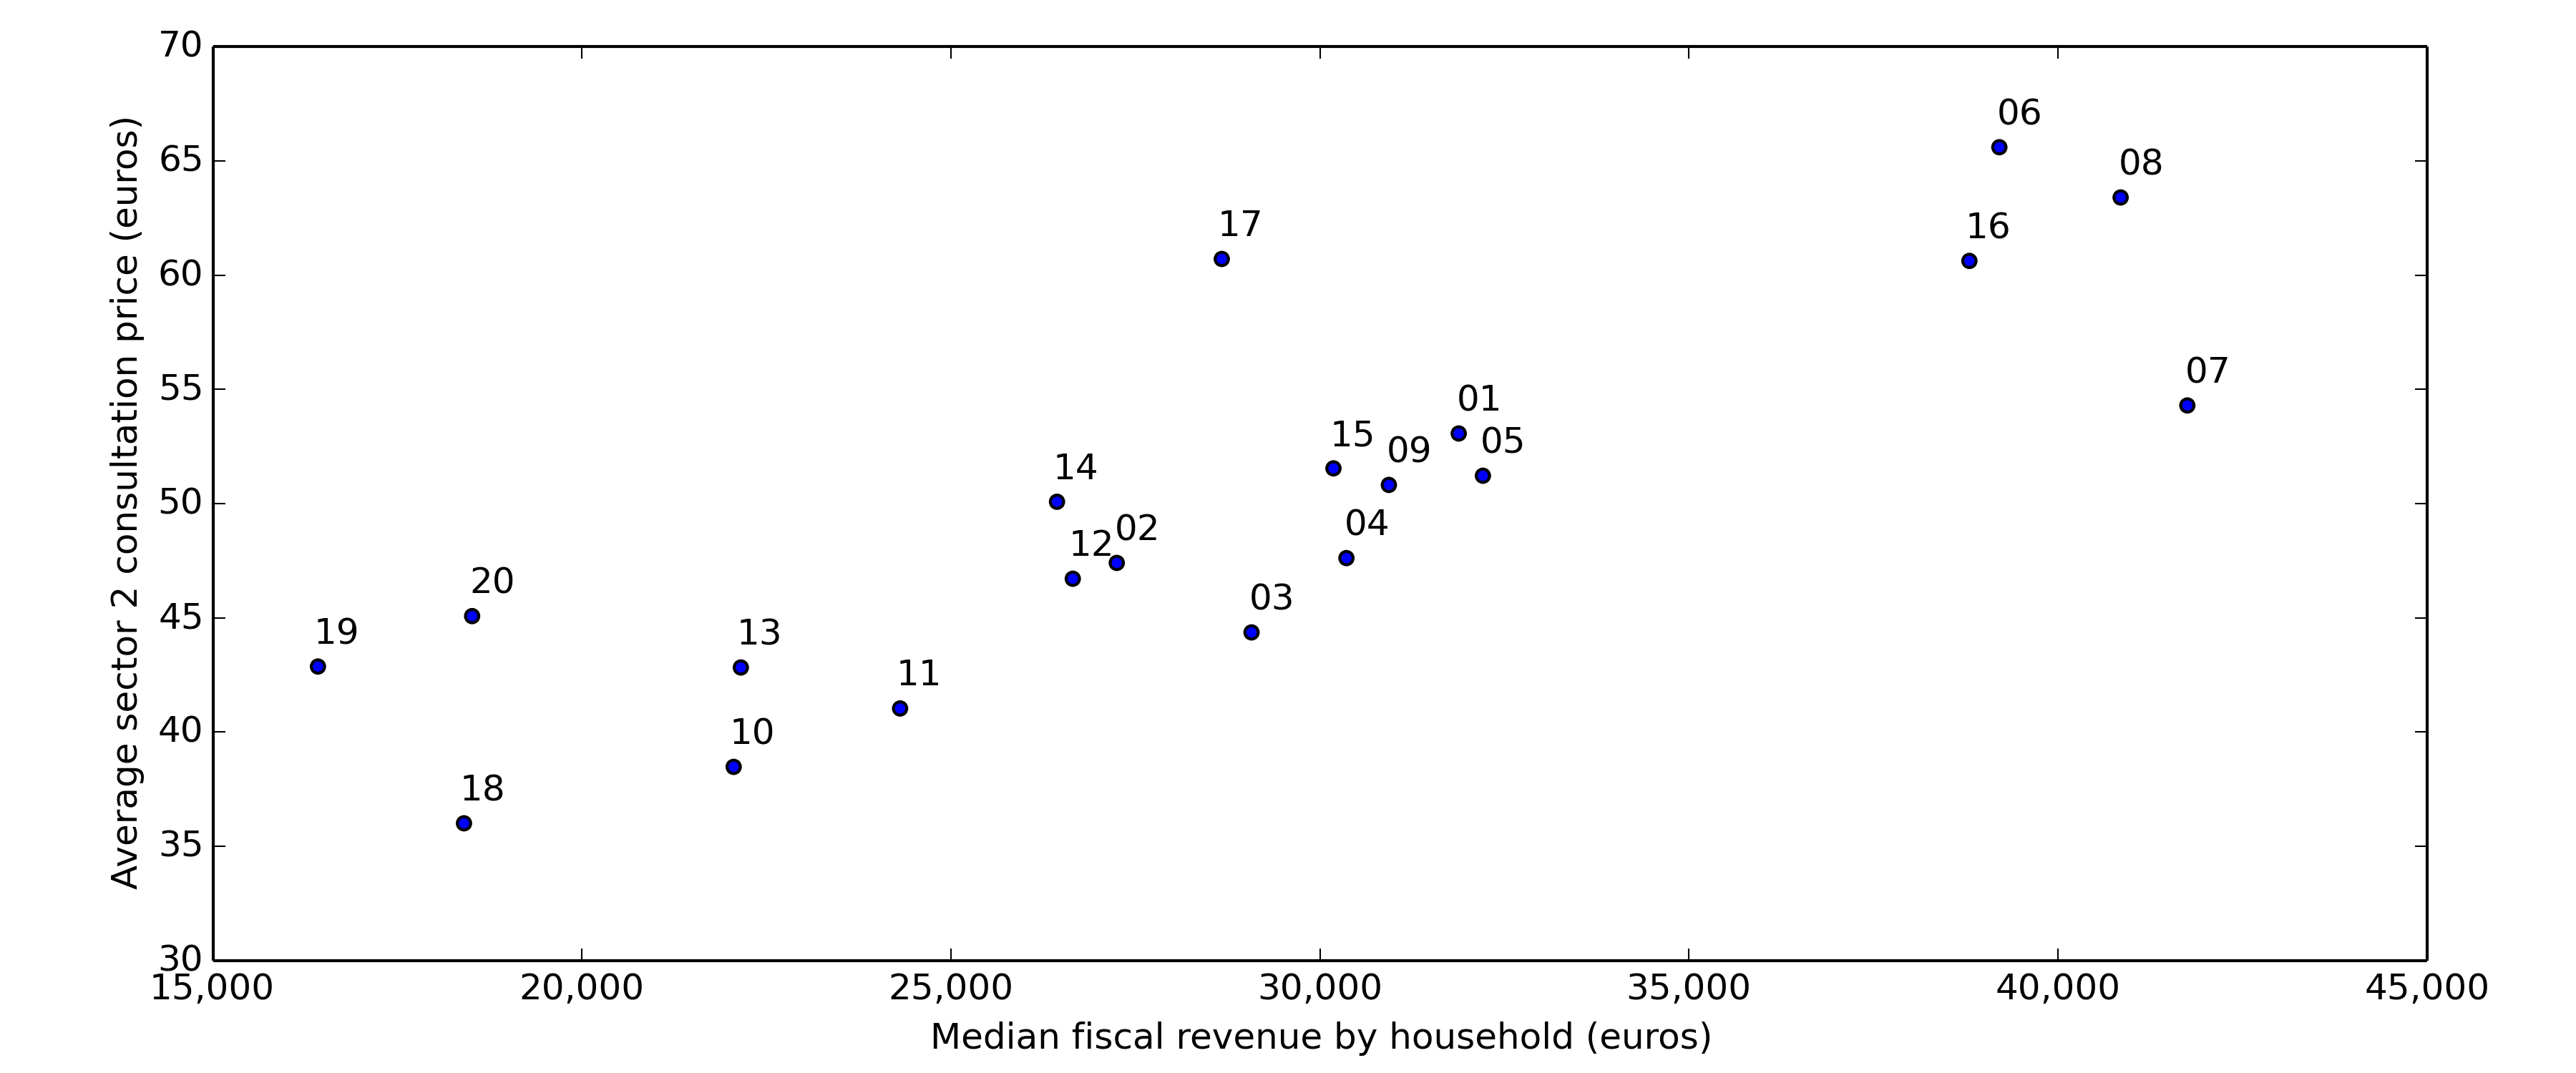
\includegraphics[width=16cm]{images/GP_Ardt_ConsultationS2VsRevenue.png}
\end{figure}

\section{Ophtalmologists}

ADD TABLE: NBS (STATUS), DENSITY, AVG PRICE

\begin{figure}[H]
    \caption{Density ophtalmologists vs. household revenue by district}
	\centering
		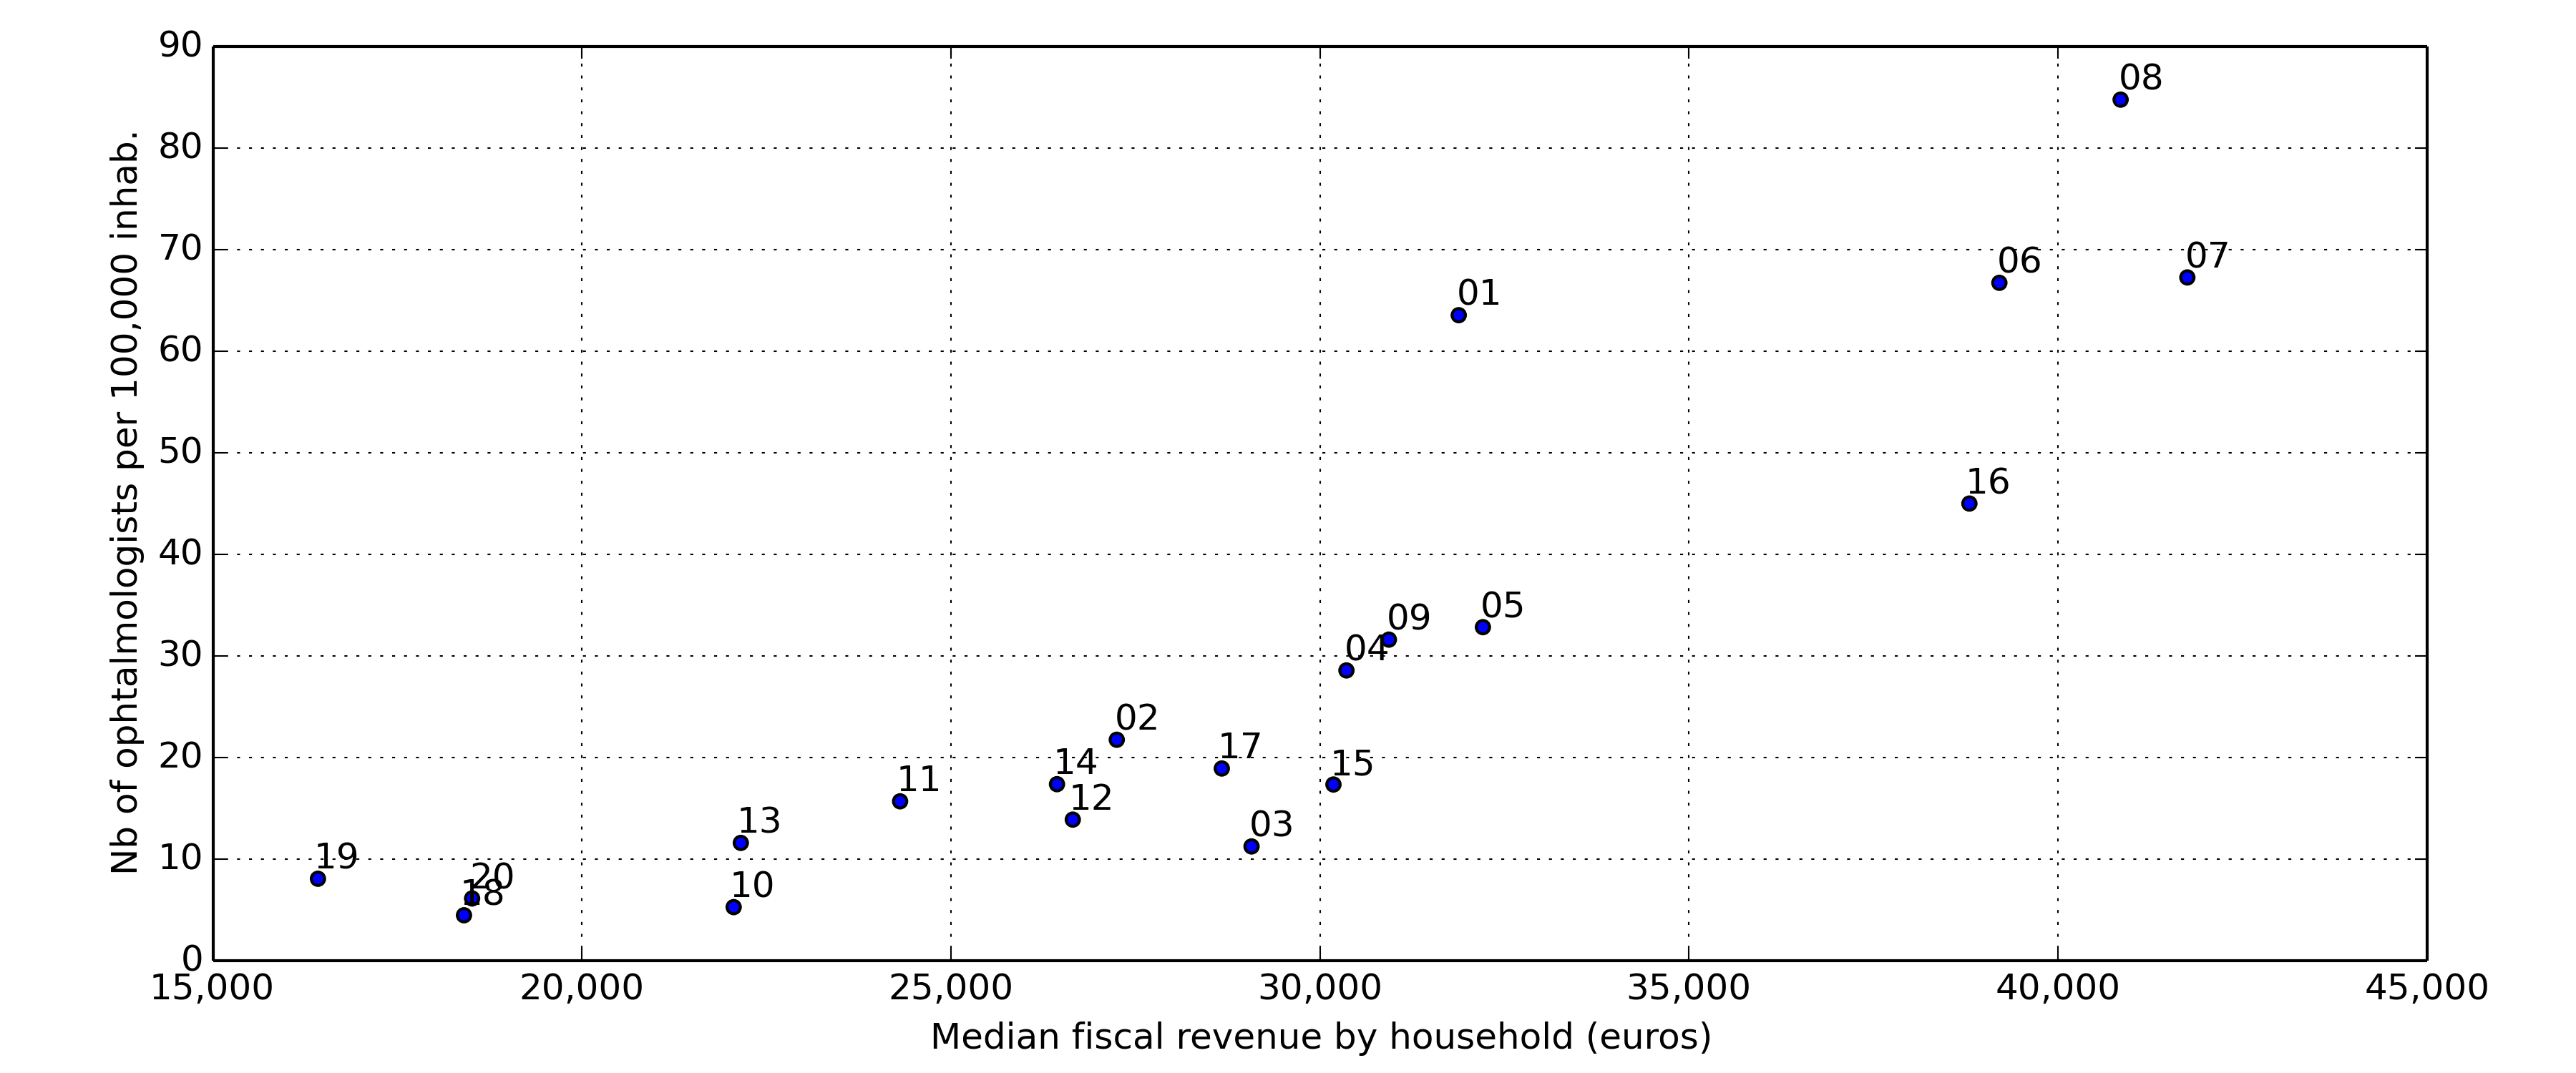
\includegraphics[width=16cm]{images/Ophtalmo_Ardt_DensityVsRevenue.png}
\end{figure}

\begin{figure}[H]
    \caption{Density of sector 1 ophtalmologists vs. household revenue by district}
	\centering
		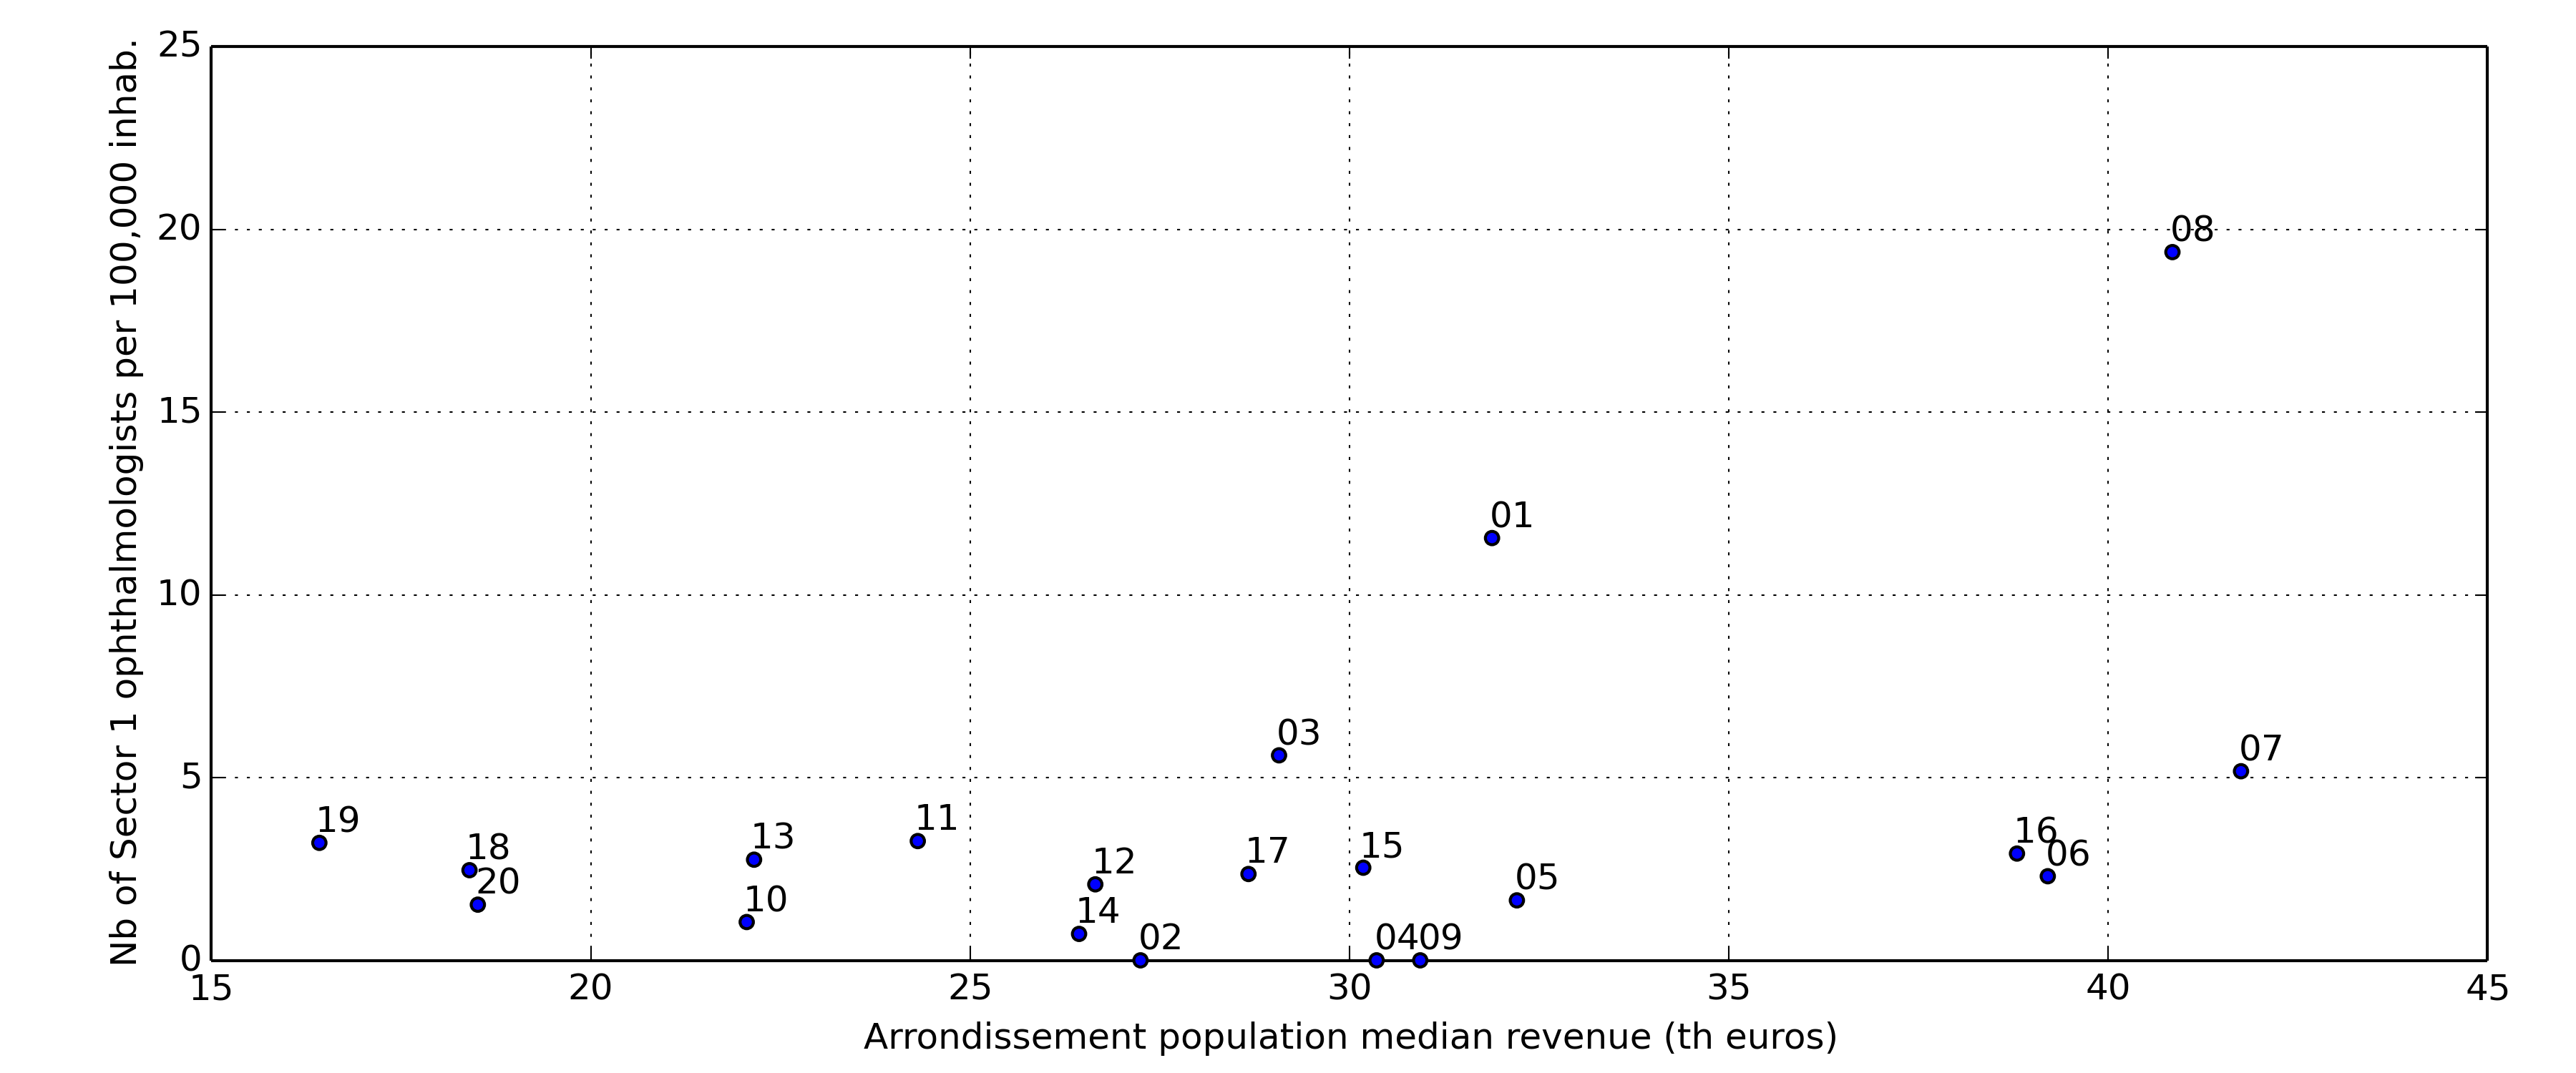
\includegraphics[width=16cm]{images/Ophtalmo_Ardt_DensityS1VsRevenue.png}
\end{figure}


\begin{figure}[H]
    \caption{Density of sector 2 ophtalmologists vs. household revenue by district}
	\centering
		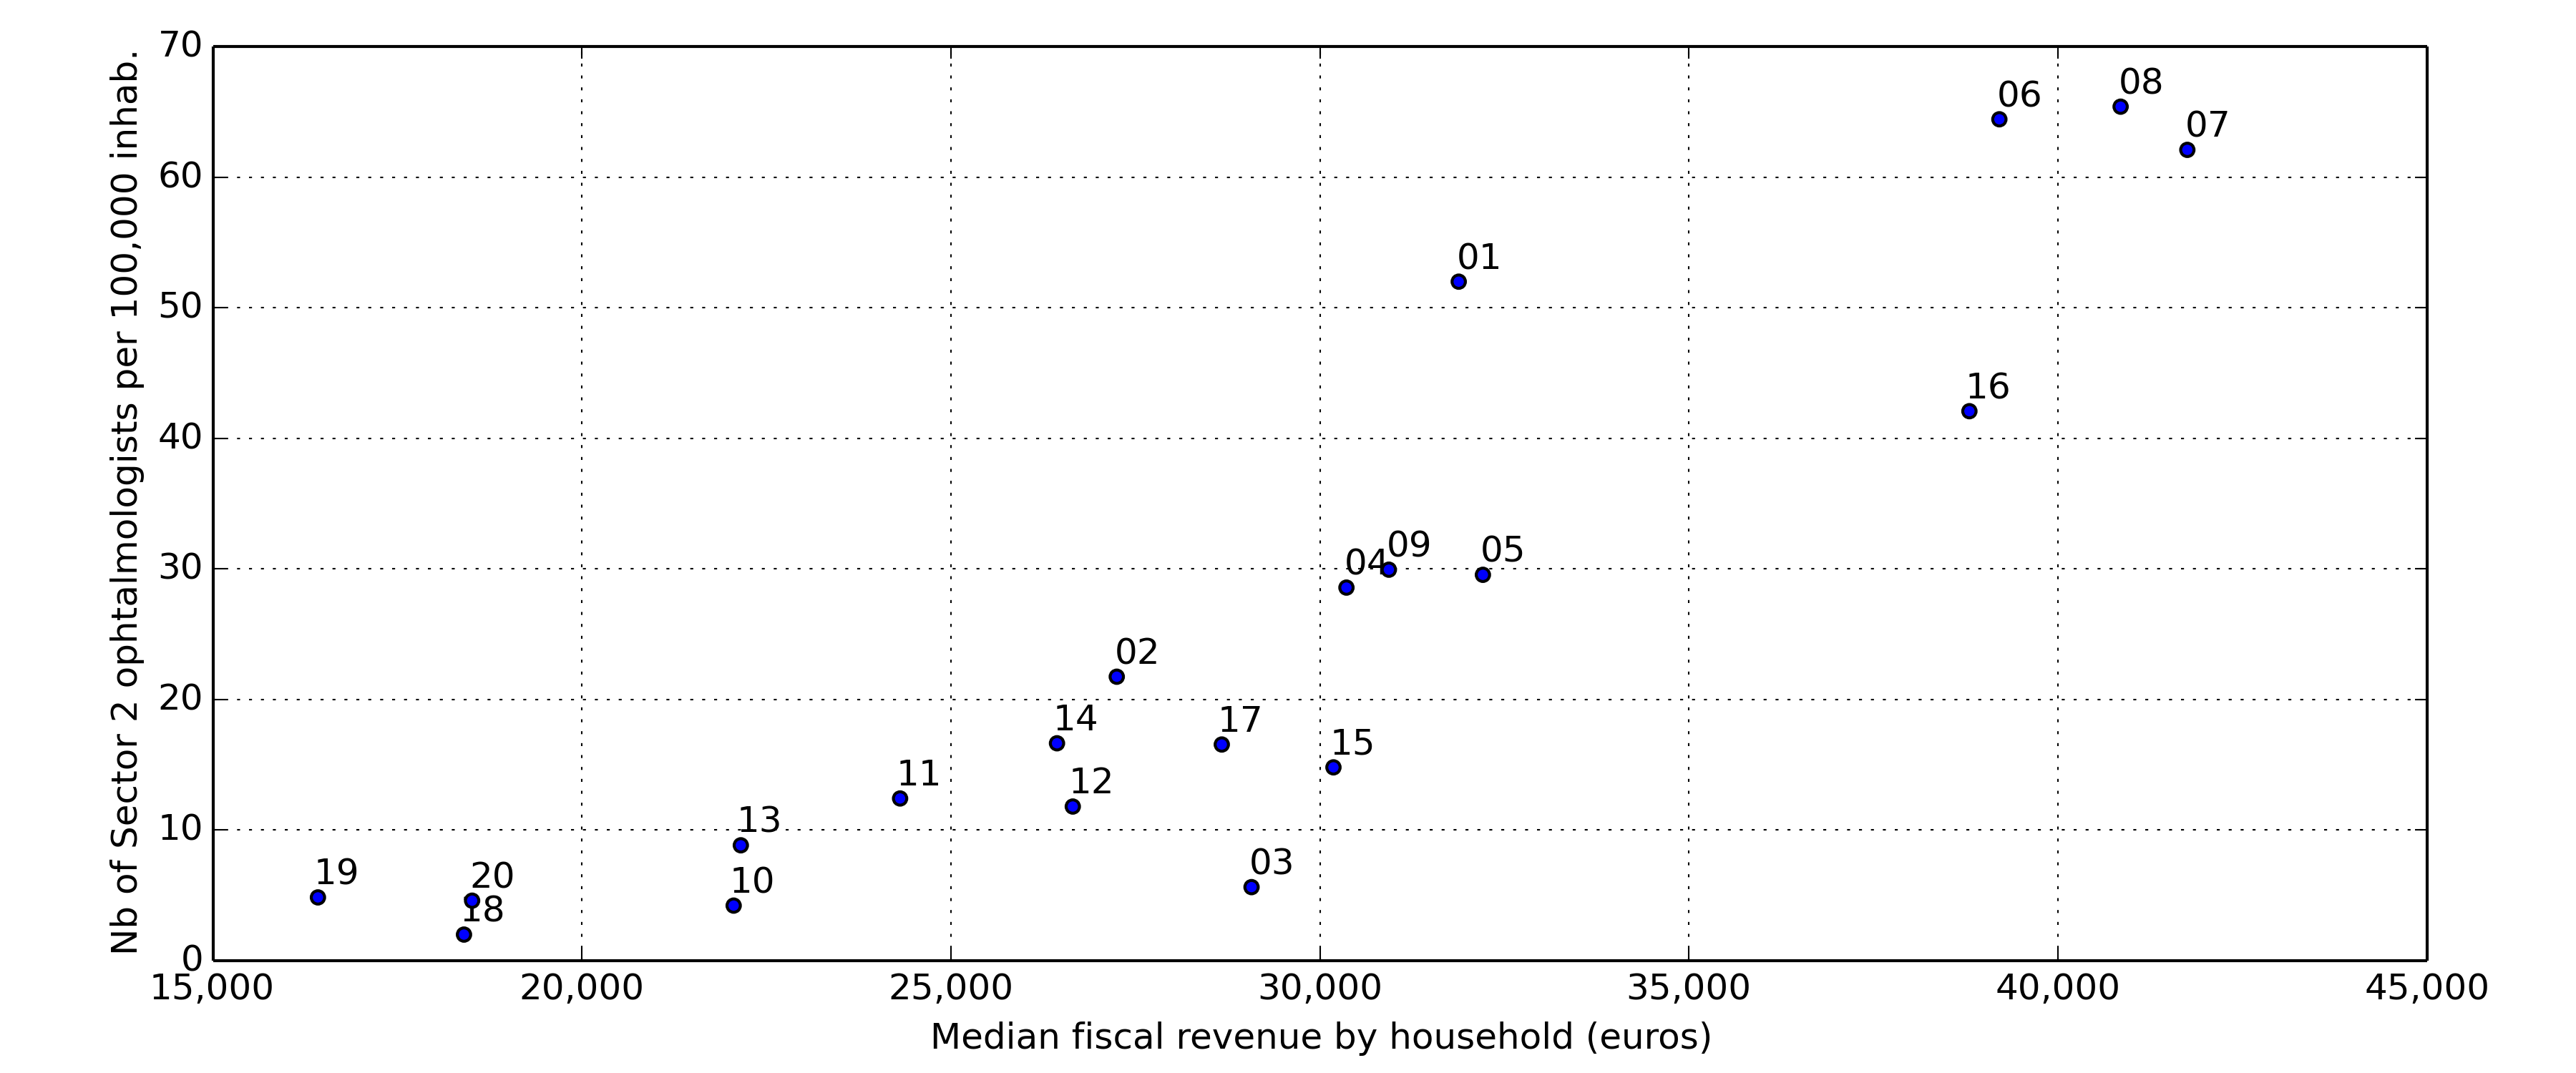
\includegraphics[width=16cm]{images/Ophtalmo_Ardt_DensityS2VsRevenue.png}
\end{figure}

\begin{figure}[H]
    \caption{Average sector 2 ophtalmologist consultation price vs. household revenue by district}
	\centering
		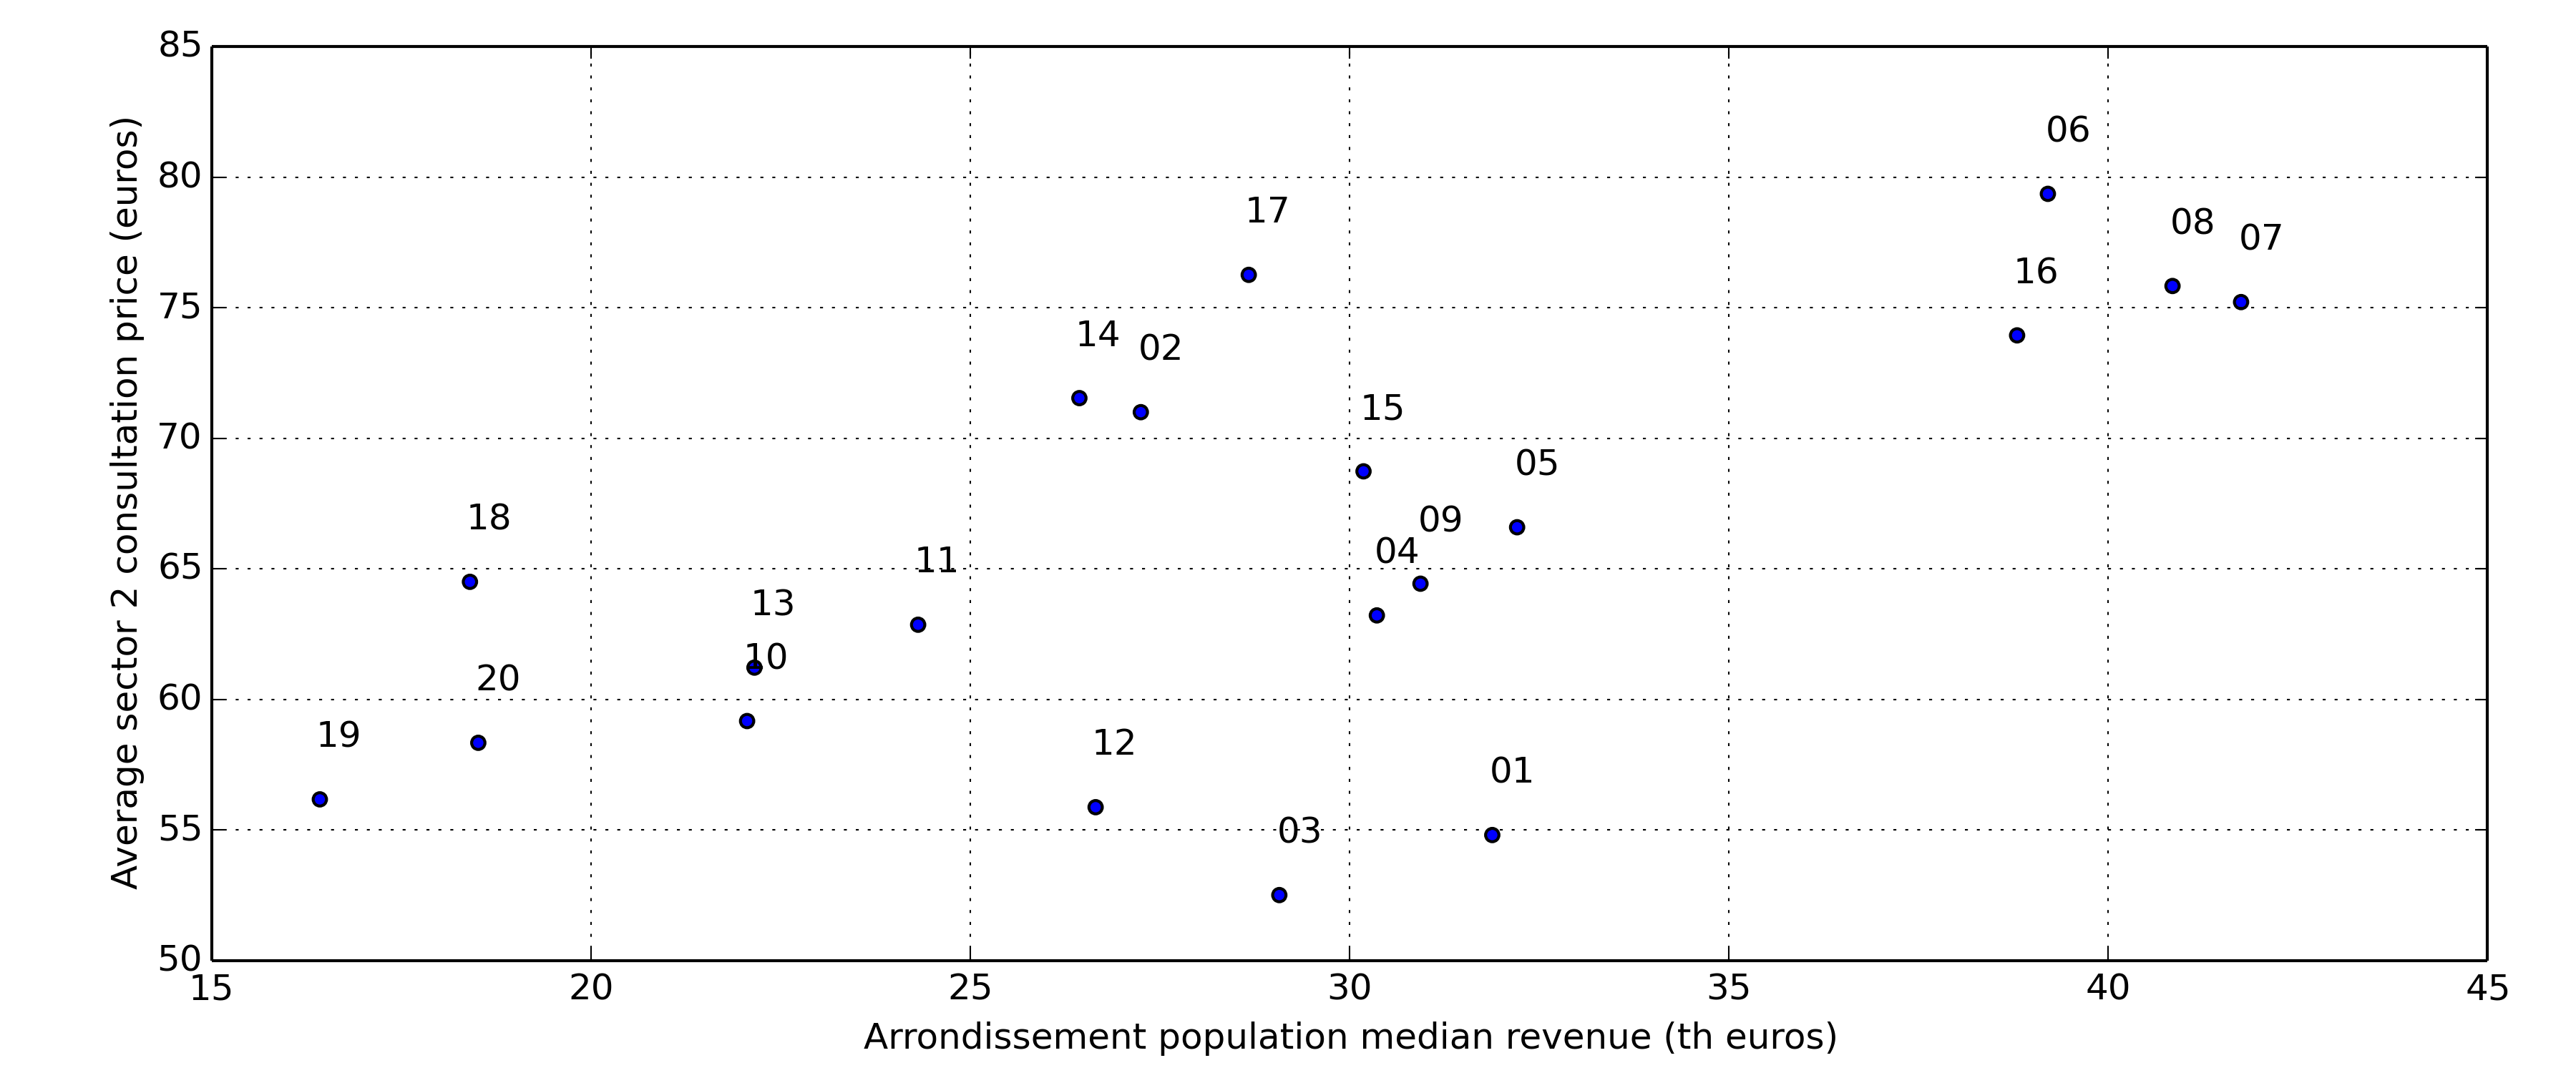
\includegraphics[width=16cm]{images/Ophtalmo_Ardt_ConsultationS2VsRevenue.png}
\end{figure}

\clearpage

\appendix


\end{document}
